% The document class supplies options to control rendering of some standard
% features in the result.  The goal is for uniform style, so some attention 
% to detail is *vital* with all fields.  Each field (i.e., text inside the
% curly braces below, so the MEng text inside {MEng} for instance) should 
% take into account the following:
%
% - author name       should be formatted as "FirstName LastName"
%   (not "Initial LastName" for example),
% - supervisor name   should be formatted as "Title FirstName LastName"
%   (where Title is "Dr." or "Prof." for example),
% - degree programme  should be "BSc", "MEng", "MSci", "MSc" or "PhD",
% - dissertation title should be correctly capitalised (plus you can have
%   an optional sub-title if appropriate, or leave this field blank),
% - dissertation type should be formatted as one of the following:
%   * for the MEng degree programme either "enterprise" or "research" to
%     reflect the stream,
%   * for the MSc  degree programme "$X/Y/Z$" for a project deemed to be
%     X%, Y% and Z% of type I, II and III.
% - year              should be formatted as a 4-digit year of submission
%   (so 2014 rather than the academic year, say 2013/14 say).

\documentclass[ % the name of the author
                    author={Aman Kumar Singh},
                % the name of the supervisor
                supervisor={Dr. Edwin Simpson},
                % the degree programme
                    degree={MSc},
                % the dissertation    title (which cannot be blank)
                     title={Rubric-Guided Knowledge Distillation of Large Language Models for Clinically Grounded Personalised Medical Report Generation},
                % the dissertation subtitle (which can    be blank)
                  subtitle={A Quality-Aware Framework for Clinical Knowledge Transfer and Evaluation},
                % the dissertation     type
                      type={},
                % the year of submission
                      year={2021}]{dissertation}

\begin{document}

% =============================================================================

% This section simply introduces the structural guidelines.  It can clearly
% be deleted (or commented out) if you use the file as a template for your
% own dissertation: everything following it is in the correct order to use 
% as is.

\section*{Prelude}
\thispagestyle{empty}


A typical MSc thesis will be structured according to a fairly standard sequence of 
sections, and one example is shown here.  However, it is hard and perhaps even 
counter-productive to generalise: the goal of this document is {\em not}\/ to be prescriptive, to show you how you {\em must} structure your thesis; rather it is to simply to act as a guideline, to show you how you {\em could} structure your thesis.  In particular, each chapter's indicated page-count is
important but {\em not}\/ absolute: the aim is simply to highlight that a 
clear and concise description is better than a rambling alternative that makes
it hard to separate important content and facts from irrelevant trivia.

You can use this document as a \LaTeX-based 
template for your own thesis by simply deleting extraneous sections
and content, and adding your own text. If you do that, we recommend using BibTeX
to deal with the associated bibliography. 
You may want to use Overleaf (an online cloud-based collaborative \LaTeX platform).


The words ``thesis'' and ``dissertation'' are used interchangeably here. All active hyperlinks in the PDF file are rendered in the same shade of dark blue. 



% =============================================================================

% This macro creates the standard UoB title page by using information drawn
% from the document class (meaning it is vital you select the correct degree 
% title and so on).


\maketitle

% After the title page (which is a special case in that it is not numbered)
% comes the front matter or preliminaries; this macro signals the start of
% such content, meaning the pages are numbered with Roman numerals.

\frontmatter

% This macro creates the standard UoB declaration; on the printed hard-copy,
% this must be physically signed by the author in the space indicated.

\makedecl

% LaTeX automatically generates a table of contents, plus associated lists 
% of figures, tables and algorithms.  The former is a compulsory part of the
% dissertation, but if you do not require the latter they can be suppressed
% by simply commenting out the associated macro.

\tableofcontents
\listoffigures
\listoftables
\listofalgorithms
\lstlistoflistings

% The following sections are part of the front matter, but are not generated
% automatically by LaTeX; the use of \chapter* means they are not numbered.

% -----------------------------------------------------------------------------

\chapter*{Abstract}

{\bf A compulsory section, of at most $1$ page} 
\vspace{1cm} 

\noindent
This section should summarise the project context, aims and objectives,
and main contributions (e.g., deliverables) and achievements.  The goal is to ensure that the 
reader is clear about what the topic is, what you have done within this 
topic, {\em and}\/ {\bf what your view of the outcome is.}

Essentially 
this section is a (very) short version of what is typically covered in more depth in the first 
chapter.  If appropriate, you should include here  
a clear statement of your research hypothesis.  This will obviously differ significantly
for each project, but an example might be as follows:

\begin{quote}
My research hypothesis is that a suitable genetic algorithm will yield
more accurate results (when applied to the standard ACME data set) than 
the algorithm proposed by Jones and Smith, while also executing in less
time.
\end{quote}

\noindent
The latter aspects should (ideally) be presented as a concise, factual 
list of the main points of achievement.  Again the points will differ for each project, but 
an might be as follows:

\begin{quote}
\noindent
\begin{itemize}
\item I spent $120$ hours collecting material on and learning about the 
      Java garbage-collection sub-system. 
\item I wrote a total of $5000$ lines of {\em Python} source code, and associated orchestration scripts. 
\item I designed a new algorithm for computing the non-linear mapping 
      from A-space to B-space using a genetic algorithm.
\item I implemented a version of the algorithm proposed by Jones and 
      Smith (2010), corrected a mistake in it, and 
      compared the results with several alternatives.
\end{itemize}
\end{quote}

% -----------------------------------------------------------------------------

\chapter*{Summary of Changes}

{\bf A conditional section, of at most $1$ page} 
\vspace{1cm} 

If (and only if) the dissertation represents a resubmission (e.g., as the result of
a resit), then this section is compulsory: the content should summarise all
non-trivial changes made to the initial submission.  Otherwise you can
omit it, since {\bf a summary of this type is only needed for resubmissions}.

When included, the section will ideally be used to highlight additional
work completed, and address criticism raised in any associated feedback.
Clearly it is difficult to give generic advice about how to do so, but
an example might be as follows:

\begin{quote}
\noindent
\begin{itemize}
\item Feedback from the initial submission criticised the design and 
      implementation of my genetic algorithm, stating ``there seems 
      to have been no attention to computational complexity during the
      design, and obvious methods of optimisation are missing within
      the resulting implementation''.  Chapter 3 now includes a
      comprehensive analysis of the algorithm, in terms of both time
      and space.  While I have not altered the algorithm itself, I
      have included a cache mechanism (also detailed in Chapter 3)
      that provides a significant improvement in average run-time.
\item I added a feature in my implementation to allow automatic rather
      than manual selection of various parameters; the experimental
      results in Chapter 4 have been updated to reflect this.
\item Questions after the presentation highlighted a range of related
      work that I had not considered: I have make a number of updates 
      to Chapter 2, resolving this issue.
\end{itemize}
\end{quote}

% -----------------------------------------------------------------------------

\chapter*{Supporting Technologies}

{\bf A compulsory section, of at most $1$ page}
\vspace{1cm} 

\noindent
This section should present a detailed summary, in bullet point form, 
of any third-party resources (e.g., hardware and software components) 
used during the project.  Use of such resources is always perfectly 
acceptable: the goal of this section is simply to be clear about how
and where they are used, so that a clear assessment of your work can
result.  The content can focus on the project topic itself (rather,
for example, than including ``I used \mbox{\LaTeX} to prepare my 
dissertation''); an example is as follows:

\begin{quote}
\noindent
\begin{itemize}

\item I used the {\em Pandas} and {\em Seaborn} public-domian Python Libraries. 

\item I used a parts of the OpenCV computer vision library to capture 
      images from a camera, and for various standard operations (e.g., 
      threshold, edge detection).

\item I used Amazon Web Services for remote storage and processing of data. Specifically, I used:
 \begin{itemize}
 \item Simple Storage Service (S3) for data storage
 \item Elastic Compute Cloud (EC2) for provision of virtual machines
 \item Elastic Beanstalk for scaling and load management
 \item Sagemaker for all the machine learning components of my project. 
 \end{itemize}
 
\item I used \LaTeX\ to format my thesis, via the online service {\em Overleaf}. 
\end{itemize}
\end{quote}

% -----------------------------------------------------------------------------

\chapter*{Notation and Acronyms}

{\bf An optional section, of roughly $1$ or $2$ pages}
\vspace{1cm} 

\noindent
Any well written document will introduce notation and acronyms before
their use, {\em even if} they are standard in some way: this ensures 
any reader can understand the resulting self-contained content.  

Said introduction can exist within the dissertation itself, wherever 
that is appropriate.  For an acronym, this is typically achieved at 
the first point of use via ``Advanced Encryption Standard (AES)'' or 
similar, noting the capitalisation of relevant letters.  However, it 
can be useful to include an additional, dedicated list at the start 
of the dissertation; the advantage of doing so is that you cannot 
mistakenly use an acronym before defining it.  A limited example is 
as follows:

\begin{quote}
\noindent
\begin{tabular}{lcl}
AES                 &:     & Advanced Encryption Standard                                         \\
DES                 &:     & Data Encryption Standard                                             \\
                    &\vdots&                                                                      \\
${\mathcal H}( x )$ &:     & the Hamming weight of $x$                                            \\
${\mathbb  F}_q$    &:     & a finite field with $q$ elements                                     \\
$x_i$               &:     & the $i$-th bit of some binary sequence $x$, st. $x_i \in \{ 0, 1 \}$ \\
\end{tabular}
\end{quote}

% -----------------------------------------------------------------------------

\chapter*{Acknowledgements}

{\bf An optional section, of at most $1$ page}
\vspace{1cm} 

\noindent
It is common practice (although totally optional) to acknowledge any
third-party advice, contribution or influence you have found useful
during your work.  Examples include support from friends or family, 
the input of your Supervisor and/or Advisor, external organisations 
or persons who  have supplied resources of some kind (e.g., funding, 
advice or time), and so on.

\vspace{1cm}
Dave Cliff writes here to say huge thanks to his colleague Dr Dan Page for sharing this \LaTeX\ thesis template, which was originally written by Dan, for Computer Science dissertations. Dave edited Dan's original to better suit the needs of the Data Science MSc: please don't hassle Dan about any of this, but do feel free to contact Dave if you have any questions or comments on it.  

% =============================================================================

% After the front matter comes a number of chapters; under each chapter,
% sections, subsections and even subsubsections are permissible.  The
% pages in this part are numbered with Arabic numerals.  Note that:
%
% - A reference point can be marked using \label{XXX}, and then later
%   referred to via \ref{XXX}; for example Chapter\ref{chap:context}.
% - The chapters are presented here in one file; this can become hard
%   to manage.  An alternative is to save the content in seprate files
%   the use \input{XXX} to import it, which acts like the #include
%   directive in C.

\mainmatter

% -----------------------------------------------------------------------------

\chapter{Introduction}
\label{chap:introduction}

{\bf A compulsory chapter, roughly 10\% of the total page-count}
\vspace{1cm} 

% putting a \noindent before the first para in each chapter looks nicer.
\noindent
This chapter should describe the project context, and motivate each of
the proposed aims and objectives.  Ideally, it is written at a fairly 
high-level, and easily understood by a reader who is technically 
competent but not an expert in the topic itself.

In short, the goal is to answer three questions for the reader.  First, 
what is the project topic, or problem being investigated?  Second, why 
is the topic important, or rather why should the reader care about it?  
For example, why there is a need for this project, who will benefit from the 
project and in what way (e.g., clients/end-users who needed some analysis
done, or other data scientists who might need the tools you have developed), what 
work does the project build on and why is the selected approach either
important and/or interesting (e.g., fills a gap in literature, applies
results from another field to a new problem).  Finally, what are the 
central challenges involved and why are they significant? 
 
The chapter should conclude with a concise bullet point list that 
summarises the aims, objectives, {\bf and achievements}\/ of your work. 

% -----------------------------------------------------------------------------

\chapter{Background}
\label{chap:background}
\section{Personalised Medical Reports in Neurogenetic Disorders}
\subsection{Neurogenetic and Neurodevelopmental Disorders}
Neurodevelopmental disorders (NDDs) are a heterogeneous group of conditions that emerge during childhood and affect brain development and functioning, often resulting in difficulties with cognition, communication, behaviour, learning, and social functioning. Genetic factors contribute substantially to many NDDs, leading to considerable variation in symptoms, severity, and combinations of intellectual, behavioural, motor, and neurological features \cite{gao_genetic_2025, assadourian_precision_2025}.

KBG syndrome (KBGS) is a rare genetic neurodevelopmental disorder primarily associated with pathogenic variants or deletions involving the ANKRD11 gene. It presents with a broad spectrum of features, including developmental delay, intellectual and learning difficulties, behavioural and neurological abnormalities, distinctive craniofacial features, macrodontia, short stature, and skeletal abnormalities \cite{martinez-cayuelas_clinical_2023}. The combination and severity of these features can vary substantially between children, highlighting the need to represent each child's individual clinical profile rather than relying solely on generic descriptions.

For families, understanding rare genetic disorders can be challenging due to limited condition-specific information and complex medical terminology. Personalised and accessible patient reports can help consolidate information about a child's symptoms, medical history, and care needs into a clear, patient-specific summary, supporting parents in understanding their child's condition and communicating with healthcare professionals \cite{low_identifying_2025, burbury_exploring_2025}. This motivates the use of automated patient report generation to produce personalised, understandable summaries from complex clinical and background information.

\subsection{LLM-Based Personalised Medical Report Generation}
Large Language Models (LLMs), such as GPT-4o and BioGPT, have demonstrated strong capabilities in medical report generation, clinical summarisation, and healthcare documentation, highlighting their potential to synthesise complex clinical information \cite{yuan_continued_2024, rehman_advancement_2025, alabed_large_2026, che_llm-driven_2026, makram_ai_2024}. These capabilities make LLMs promising for personalised patient report generation, as they can integrate patient-specific information and generate summaries tailored to individual clinical contexts. For example, Ganzinger et al. \cite{ganzinger_automated_2025} used open-source LLMs to generate German discharge summaries from structured EHR data, while Tariq et al. \cite{tariq_patient_2024} developed a patient-sensitive model for generating radiology summaries adapted to different levels of medical knowledge. These studies demonstrate the potential of LLMs for generating both clinically useful and patient-oriented medical reports.
\subsection{Challenges of LLM-Based Patient Report Generation}
Despite their potential, deploying large, cloud-hosted LLMs in clinical settings presents significant privacy, regulatory, and resource challenges. Patient–doctor consultations contain highly sensitive medical information, while regulations such as HIPAA and GDPR restrict the transfer of clinical data to external commercial APIs, raising important privacy and compliance concerns \cite{annas_hipaa_2003, noauthor_eu_nodate, zhong_considerations_2025, al-dhabyani_data_2026}. Furthermore, many community clinics and regional hospitals have limited computational resources and may lack the specialised GPU infrastructure required to locally deploy and efficiently run large open-weight models \cite{li_collm_2024}.

\subsection{SLM-Based Personalised Medical Report Generation}
Small Language Models (SLMs) have emerged as efficient alternatives to large language models (LLMs), offering lower computational, memory, and storage requirements while maintaining competitive performance on domain-specific tasks \cite{wang_comprehensive_2025, garg_rise_2026}. These advantages make SLMs attractive for healthcare, where local deployment can improve privacy and reduce reliance on cloud infrastructure when processing sensitive patient information \cite{wang_comprehensive_2025}.

SLMs have demonstrated potential in medical applications. For example, Meerkat showed improved reasoning performance across medical benchmarks while maintaining a lightweight architecture \cite{kim_small_2025}, while Rohanian et al. \cite{rohanian_effectiveness_2022} developed lightweight biomedical models that achieved performance comparable to larger models on downstream tasks. This suggests that SLMs can support clinical text processing and generation with more practical deployment requirements.

For personalised patient report generation, SLMs could enable patient-specific clinical information to be processed locally, reducing the need to transmit sensitive data to external APIs. However, their smaller size can limit complex reasoning and specialised medical knowledge \cite{turki_evaluating_2025, wang_comprehensive_2025}. Knowledge distillation can address this limitation by transferring useful capabilities from larger teacher models to smaller student models \cite{gou_knowledge_2021}.
\section{Knowledge Distillation}
\subsection{Fundamentals of Knowledge Distillation}
Knowledge distillation (KD) is a model compression and knowledge-transfer technique in which a smaller student model learns useful knowledge from a larger and more capable teacher model \cite{hinton_distilling_2015, wang_knowledge_2022}. Unlike conventional compression approaches such as pruning, quantisation, and low-rank factorisation, which reduce or modify the model's parameters or architecture, KD transfers knowledge from the teacher to the student without necessarily altering the underlying model architecture \cite{wang_knowledge_2022, mansourian_comprehensive_2025}. The teacher provides additional learning signals, such as its output distributions, allowing the student to learn aspects of the teacher's behaviour beyond conventional hard target labels \cite{hinton_distilling_2015}.

The central principle of KD is therefore knowledge transfer, whereby information learned by a large model is transferred to a smaller model during training. This enables the student to acquire useful capabilities of the teacher while retaining the computational and memory advantages of a smaller architecture. Consequently, KD can reduce the resources required for model inference and deployment while aiming to preserve much of the teacher's predictive or generative performance \cite{hinton_distilling_2015, wang_knowledge_2022}. Beyond model compression, KD can also facilitate knowledge transfer when labelled data are limited or when knowledge must be transferred across different tasks or models. In privacy-sensitive settings, data-free distillation provides another alternative by enabling knowledge transfer without directly requiring access to the original training data \cite{wang_knowledge_2022}.

The effectiveness of KD depends on several design choices, including what knowledge is transferred, how this knowledge is transferred, and how the teacher and student models are configured \cite{mansourian_comprehensive_2025}. These considerations have led to a range of distillation approaches based on different teacher–student configurations and forms of transferred knowledge, which are discussed in the following subsection.
\begin{figure}[htbp]
    \centering
    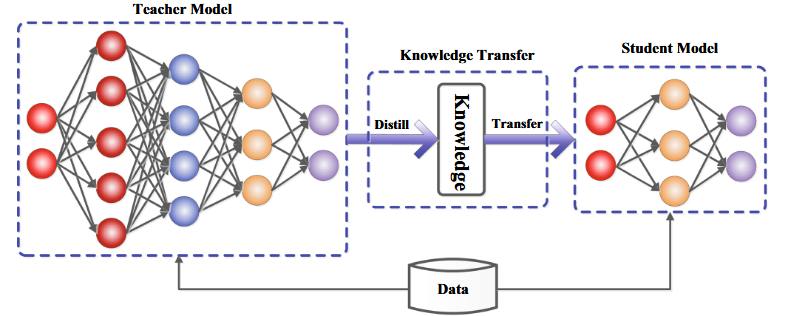
\includegraphics[width=0.7\textwidth]{Screenshot 2026-08-11 162229.png}
    \caption{Generic teacher--student framework for knowledge distillation \cite{gou_knowledge_2021}.}
    \label{fig:kd}
\end{figure}
\subsection{Types of Knowledge Distillation}
Knowledge distillation can be categorised according to the training strategy, accessibility of the teacher model, and type of knowledge transferred. These classifications describe different aspects of the teacher–student framework and are not mutually exclusive.
\subsubsection{Offline, Online, and Self-Distillation}
Offline distillation is the most common form of knowledge distillation and typically involves a pretrained teacher model whose parameters remain frozen while a smaller student learns from its outputs \cite{hinton_distilling_2015, wang_knowledge_2022}. Although straightforward and effective, it requires the teacher to remain available during student training and may transfer biases or limitations present in the teacher \cite{guo_reducing_2021, huang_knowledge_2022-1}.

In online distillation, the teacher and student are trained simultaneously, allowing knowledge to be transferred dynamically during the training process \cite{chen_online_2020}. The teacher may be constructed from multiple student models or branches, removing the need for a separately pretrained teacher, although this can increase training complexity. Self-distillation is a related approach in which knowledge is transferred within the same model, such as from an earlier training stage, deeper layer, or previous version of the model \cite{furlanello_born_2018, zhang_be_2019}. It can improve model performance without requiring a separate, larger teacher network.

\subsubsection{Black-Box and White-Box Distillation}
White-box distillation assumes access to the teacher model's internal information, such as logits, hidden representations, attention patterns, or model parameters. This allows the student to learn from richer signals than the teacher's final outputs, but requires access to the teacher's internal architecture and computations \cite{donisch_inference_2024}.

In contrast, black-box distillation relies only on the teacher's externally observable outputs, without access to its internal parameters or representations. For language models, the teacher can therefore be prompted to generate responses, explanations, or rationales that are subsequently used as supervision for the student \cite{shi_knowledge_2025}. This makes black-box distillation particularly suitable for proprietary or API-based LLMs, where internal model information is inaccessible.

The key distinction is therefore the level of access to the teacher: white-box distillation exploits internal model information, whereas black-box distillation transfers knowledge primarily through the teacher's observable outputs.
\subsubsection{Response-, Logit-, and Feature-Based Distillation}
Knowledge distillation can also be classified according to the form of knowledge transferred from the teacher to the student. In response-based distillation, the student learns from the teacher's final outputs, such as predicted labels or generated text. For language models, this can involve using teacher-generated responses as training targets, making the approach particularly suitable for generative tasks \cite{yang_categories_2023}.

In logit-based distillation, the student learns from the teacher's logits or probability distributions rather than only the final predicted token. These soft targets provide information about the teacher's confidence across alternative predictions and can therefore provide richer supervision than hard labels \cite{habib_knowledge_2024}.

Feature-based distillation transfers knowledge from the teacher's intermediate representations, encouraging the student to learn similar internal features or representations. This can provide richer information about how the teacher processes the input, although it generally requires access to the teacher's internal architecture \cite{park_relational_2019}.
\subsection{Knowledge Distillation for LLMs}
Knowledge distillation for language models extends the teacher–student framework to generative tasks, where a smaller student model learns to reproduce useful capabilities of a larger teacher model. Rather than transferring knowledge for a single prediction task, the process aims to transfer aspects of the teacher's language generation, instruction following, domain knowledge, and response structure \cite{chen_distilling_2021}.

A common approach is to use a teacher LLM to generate instruction–response pairs or synthetic training examples, which are then used to fine-tune the student model\cite{wang_self-instruct_2023}. This provides a practical way of transferring capabilities from large, computationally expensive models to smaller models that are more suitable for efficient deployment. It is particularly useful when the teacher is proprietary or accessed through an API, as the student can be trained using the teacher's generated outputs without requiring access to its internal architecture.

However, distillation of generative language models introduces important challenges. Errors, hallucinations, and undesirable behaviours in teacher-generated responses may be transferred to the student, while the smaller model may not have sufficient capacity to reproduce the full range of the teacher's capabilities\cite{zhang_lifting_2023}. Therefore, the quality and relevance of the teacher-generated training data become important determinants of student performance . This is particularly critical in clinical report generation, where generated content must be accurate, coherent, relevant, and grounded in the individual patient's information. These considerations motivate the need for quality-aware approaches to knowledge distillation, discussed in the following section.
\subsection{Research Gap and Proposed Rubric-Weighted Knowledge Distillation}
.\\
.\\
.\\
.\\
.\\
.\\
.\\
.\\
.\\
.\\
.\\
.\\
.\\
.\\
.\\
.\\
.\\
.\\
.\\
.\\
.\\
.\\
.\\
.\\
.\\
.\\
.\\
.\\
.\\
.\\
.\\
.\\
.\\
.\\
.\\
.\\
.\\
.\\
.\\
.\\
.\\
.\\
\section{Evaluation}
The evaluation of generated clinical reports requires multiple complementary measures, as no single metric captures all aspects of quality. This study evaluates clinical and linguistic quality, similarity to reference or teacher-generated reports, and model efficiency.
\subsection{Clinical Report Quality Dimensions}
Clinical report quality encompasses multiple dimensions that assess both the accuracy of the generated information and the effectiveness of its presentation. In this study, five key dimensions are considered: factuality, coverage, conciseness, readability, and medical tone, each capturing a distinct aspect of report quality. The following provides a brief description of each dimension.\\
\textbf{Factuality:} Whether the generated report accurately reflects the provided clinical information without false, contradictory, or unsupported claims \cite{munnangi_factehr_2025}.\\
\textbf{Coverage:} Whether the generated report is supported by and adequately represents the relevant information provided in the source \cite{moramarco_towards_2021}.\\
\textbf{Conciseness:} Whether the report communicates relevant information clearly and efficiently without unnecessary repetition, irrelevant content, or excessive detail \cite{schoonbeek_quality_2025}.\\
\textbf{Readability:} Whether the report is clear, coherent, and easy for the intended audience to understand.
\textbf{Medical Tone:} Whether the report uses professional, clinically appropriate, and audience-suitable language \cite{seo_evaluation_2024}.

\subsection{Rubric-Based and LLM-as-a-Judge Evaluation}
Rubric-based evaluation uses a predefined set of criteria and scoring guidelines, known as a rubric, to systematically assess generated reports. Each report is evaluated across specific quality dimensions using the same criteria, enabling consistent and structured assessment of different aspects of report quality. This allows complex qualitative properties, such as factuality and readability, to be represented through standardised scores \cite{hashemi_llm-rubric_2024}. Rubrics are particularly useful for generated clinical reports, where quality is inherently multidimensional and cannot be adequately captured by a single metric. A multidimensional rubric allows these aspects to be assessed independently while providing a common framework across different outputs. Furthermore, rubrics can guide automated evaluation by providing an LLM with explicit criteria for assessing generated reports, reducing the need for manual assessment and enabling evaluation of large collections of outputs \cite{fan_sedareval_2024}.

LLM-as-a-Judge extends this approach by using a language model to evaluate generated reports according to the predefined rubric. The judge assesses each report across the specified dimensions and assigns corresponding scores, enabling scalable evaluation while capturing qualitative properties that may be difficult to measure using conventional automatic metrics \cite{zheng_judging_2023}. In clinical report generation, this approach provides a unified framework for assessing dimensions such as factuality, coverage, conciseness, readability, and medical tone.

Despite its scalability and flexibility, LLM-as-a-Judge evaluation presents several challenges. Its reliability depends on the clarity and design of the rubric, as ambiguous criteria may lead to inconsistent scoring. The judging model may also exhibit evaluator bias or produce variable scores across evaluation runs \cite{pombal_self-preference_2026}. In clinical settings, an additional challenge is the ability to identify subtle medical errors and distinguish clinically supported information from statements that are merely plausible. Therefore, clearly defined rubrics and consistent evaluation procedures are important for obtaining reliable and meaningful assessment scores.
\subsection{Automatic Evaluation and Model Efficiency}
Automatic evaluation metrics provide quantitative measures that complement rubric-based assessment. Text similarity metrics, such as ROUGE \cite{lin_rouge_2004}, BLEU \cite{ward_bleu_2001}, BERTScore \cite{zhang_bertscore_2020}, and embedding-based semantic similarity, assess the lexical or semantic correspondence between generated reports and reference or teacher-generated reports. While lexical metrics focus on word or phrase overlap, semantic metrics capture similarities in meaning despite differences in wording. Model efficiency is also important when evaluating an SLM, particularly in resource-constrained settings. Measures such as parameter count, inference time, memory usage, and token generation speed indicate the model's computational cost and practical deployability \cite{wani_benchmarking_2026}. Together, these measures provide a broader assessment of both report quality and model performance.


\chapter{Execution}
\label{chap:execution}

{\bf A topic-specific chapter, roughly 30\% of the total page-count}
\vspace{1cm} 

\noindent
This chapter is intended to describe what you did: the goal is to explain
the main activity or activities, of any type, which constituted your work 
during the project.  The content is highly topic-specific. For some 
projects it will make sense to split the content into two main sections, or maybe even into two separate chapters: one 
will discuss the design of something, including any rationale or decisions made, 
and the other will discuss how this design was realised via some form of 
implementation.  You could instead give this chapter the title ``Design and Implementation"; or you might split this content into two chapters, one titled ``Design" and the other ``Implementation" .

Note that it is common to include evidence of ``best practice'' project 
management (e.g., use of version control, choice of programming language 
and so on).  Rather than simply a rote list, make sure any such content 
is useful and/or informative in some way: for example, if there was a 
decision to be made then explain the trade-offs and implications 
involved.

\section{Example Section}

This is an example section; 
the following content is auto-generated dummy text.
\lipsum

\subsection{Example Sub-section}

\begin{figure}[t]
\centering
foo
\caption{This is an example figure.}
\label{fig}
\end{figure}

\begin{table}[t]
\centering
\begin{tabular}{|cc|c|}
\hline
foo      & bar      & baz      \\
\hline
$0     $ & $0     $ & $0     $ \\
$1     $ & $1     $ & $1     $ \\
$\vdots$ & $\vdots$ & $\vdots$ \\
$9     $ & $9     $ & $9     $ \\
\hline
\end{tabular}
\caption{This is an example table.}
\label{tab}
\end{table}

\begin{algorithm}[t]
\For{$i=0$ {\bf upto} $n$}{
  $t_i \leftarrow 0$\;
}
\caption{This is an example algorithm.}
\label{alg}
\end{algorithm}

\begin{lstlisting}[float={t},caption={This is an example listing.},label={lst},language=C]
for( i = 0; i < n; i++ ) {
  t[ i ] = 0;
}
\end{lstlisting}

This is an example sub-section;
the following content is auto-generated dummy text.
Notice the examples in Figure~\ref{fig}, Table~\ref{tab}, Algorithm~\ref{alg}
and Listing~\ref{lst}.
\lipsum

\subsubsection{Example Sub-sub-section}

This is an example sub-sub-section;
the following content is auto-generated dummy text.
\lipsum

\paragraph{Example paragraph.}

This is an example paragraph; note the trailing full-stop in the title,
which is intended to ensure it does not run into the text.

% -----------------------------------------------------------------------------

\chapter{Critical Evaluation}
\label{chap:evaluation}

{\bf A topic-specific chapter, roughly 30\% of the total page-count} 
\vspace{1cm} 

\noindent
This chapter is intended to evaluate what you did.  The content is highly 
topic-specific, but for many projects will have flavours of the following:

\begin{enumerate}
\item functional  testing, including analysis and explanation of failure 
      cases,
\item behavioural testing, often including analysis of any results that 
      draw some form of conclusion wrt. the aims and objectives,
      and
\item evaluation of options and decisions within the project, and/or a
      comparison with alternatives.
\end{enumerate}

\noindent
This chapter often acts to differentiate project quality: even if the work
completed is of a high technical quality, critical yet objective evaluation 
and comparison of the outcomes is crucial.  In essence, the reader wants to
learn something, so the worst examples amount to simple statements of fact 
(e.g., ``graph X shows the result is Y''); the best examples are analytical 
and exploratory (e.g., ``graph X shows the result is Y, which means Z; this 
contradicts [1], which may be because I use a different assumption'').  As 
such, both positive {\em and}\/ negative outcomes are valid {\em if} presented 
in a suitable manner.

% -----------------------------------------------------------------------------

\chapter{Conclusion}
\label{chap:conclusion}

{\bf A compulsory chapter,  roughly 10\% of the total page-count}
\vspace{1cm} 

\noindent
The concluding chapter(s) of a dissertation are often underutilized because they're 
too often left too close to the deadline: it is important to allocate enough time and 
attention to closing off the story, the narrative, of your thesis.

Again, there is no single correct way of closing a thesis. 

One good way of doing this is to have a single chapter consisting of three parts:

\begin{enumerate}
\item (Re)summarise the main contributions and achievements, in essence
      summing up the content.
\item Clearly state the current project status (e.g., ``X is working, Y 
      is not'') and evaluate what has been achieved with respect to the 
      initial aims and objectives (e.g., ``I completed aim X outlined 
      previously, the evidence for this is within Chapter Y'').  There 
      is no problem including aims which were not completed, but it is 
      important to evaluate and/or justify why this is the case.
\item Outline any open problems or future plans.  Rather than treat this
      only as an exercise in what you {\em could} have done given more 
      time, try to focus on any unexplored options or interesting outcomes
      (e.g., ``my experiment for X gave counter-intuitive results, this 
      could be because Y and would form an interesting area for further 
      study'' or ``users found feature Z of my software difficult to use,
      which is obvious in hindsight but not during at design stage; to 
      resolve this, I could clearly apply the technique of Bloggs {\em et al.}.
\end{enumerate}

Alternatively, you might want to divide this content into two chapters: a penultimate chapter with a title such as ``Further Work" and then a final chapter ``Conclusions". Again, there is no hard and fast rule, we trust you to make the right decision. 

And this, the final paragraph of this thesis template, is just a bunch of citations, added to show how to generate a BibTeX bibliography. Sources that have been randomly chosen to be cited here include:
\cite{miller_etal_2018_clojure,webber_marwan_2015,touretzky_2013_lisp,eckmann_etal_1987,marwan_2011,vach_2015,shiller_2017,vytelingum_2006,tesfatsion_2002,rust_etal_1992}.




% =============================================================================

% Finally, after the main matter, the back matter is specified.  This is
% typically populated with just the bibliography.  LaTeX deals with these
% in one of two ways, namely
%
% - inline, which roughly means the author specifies entries using the 
%   \bibitem macro and typesets them manually, or
% - using BiBTeX, which means entries are contained in a separate file
%   (which is essentially a database) then imported; this is the 
%   approach used below, with the databased being dissertation.bib.
%
% Either way, the each entry has a key (or identifier) which can be used
% in the main matter to cite it, e.g., \cite{X}, \cite[Chapter 2}{Y}.

\backmatter
\bibliographystyle{unsrt}
\bibliography{references.bib}

% -----------------------------------------------------------------------------

% The dissertation concludes with a set of (optional) appendices; these are 
% the same as chapters in a sense, but once signalled as being appendices via
% the associated macro, LaTeX manages them appropriately.

\appendix

\chapter{An Example Appendix}
\label{appx:example}

Content which is not central to, but may enhance the dissertation can be 
included in one or more appendices; examples include, but are not limited
to

\begin{itemize}
\item lengthy mathematical proofs, numerical or graphical results which 
      are summarised in the main body,
\item sample or example calculations, 
      and
\item results of user studies or questionnaires.
\end{itemize}

\noindent
Note that in line with most research conferences, the examiners are not
obliged to read such appendices.

% =============================================================================

\end{document}
